\documentclass{beamer} 
\usetheme{default} 
\usecolortheme{albatross}
\setbeamercovered{transparent}
%\useoutertheme{umbcfootline}  


\usepackage[spanish]{babel}
%\usepackage[latin1]{inputenc}
\usepackage[utf8x]{inputenc}
\usepackage{hyperref}
\usepackage{color}
\usepackage{multicol}

%\usepackage[usenames,dvipsnames]{color}
\title{Colecciones II}

\author{Manuel J. Molino Milla \and Luis Molina Garzón}

\date{\today} %

\institute{IES Virgen del Carmen \and Departamento de Informática}




%\beamerdefaultoverlayspecification{<+->}

\begin{document}


\begin{frame}
  \titlepage
\end{frame}

\begin{frame}
    \frametitle{Logo}
\begin{figure}

\includegraphics[scale=1]{imagenes/logo.jpeg} 
\caption{Logo Java}
\end{figure}
\end{frame}

%\begin{frame}
 % \frametitle{Contenido}
 %\tableofcontents[pausesections]
%\end{frame}



%\section{Framework Collection}

\begin{frame}
\frametitle{Colecciones en java}
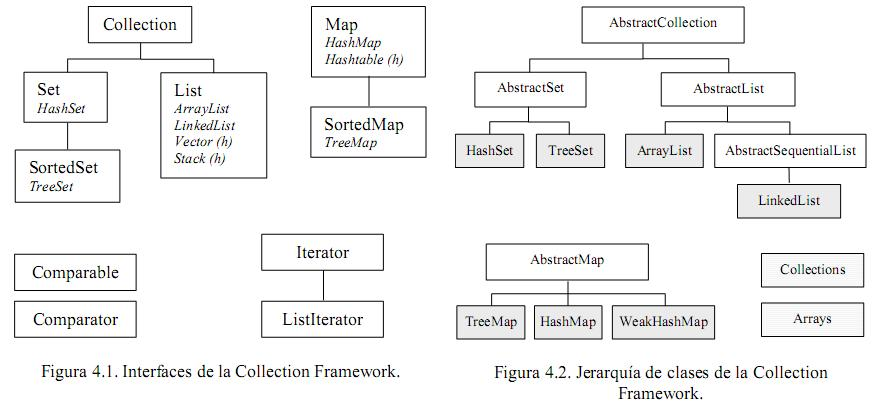
\includegraphics[scale=0.45]{imagenes/colecciones.jpeg}
\end{frame}

 
\begin{frame}[fragile]
\frametitle{Framework Collections}
\begin{itemize}[<+->]
\item Para trabajar con colecciones en Java podemos hacer uso del framework Collections.
\item Las clases e interfaces que componen este framework se encuentran en los paquetes java.util y java.util.concurrent.
\item Todas hacen uso del polimorfismo paramétrico. 
\item La raíz de la jerarquía de colecciones es la interfaz Collection$<$E$>$
\item Las más interesantes son List$<$E$>$, Set$<$E$>$ 
\item List$<E>$ contiene elementos en una secuencia concreta.
\item Set$<E>$ no puede tener elementos repetidos.
\item Otra estructura de datos que forma parte del framework, aunque no deriva de Collection$<$E$>$, dado que no se trata de una colección per se sino de un mapeo, es la que define la interfaz Map$<$E$>$, el conocido diccionario o matriz asociativa.
\end{itemize}
\end{frame}

%\subsection{Clase List}
\begin{frame}
\frametitle{Clase List}
\begin{footnotesize}
\begin{itemize}[<+->]
\item Hay varias clases que implementan la interfaz List.
\item  Las más utilizadas habitualmente son ArrayList y la vieja conocida Vector, que forma parte del framework Collections desde Java 1.2.
\item La principal diferencia entre ambas clases es que Vector es sincronizada y ArrayList no sincronizada.
\item Debido a esto no tendremos que preocuparnos de problemas de sincronización a la hora utilizar varios hilos con Vector.
\item Pero a cambio, y por la misma razón, el rendimiento de Vector es mucho peor que el de ArrayList
\item Si no necesitamos sincronización o no estamos trabajando con más de un hilo de ejecución, lo adecuado es utilizar ArrayList.
\item En todo caso, si trabajamos con varios hilos, también existe la posibilidad de sincronizar ArrayList$<$E$>$ de forma externa o utilizar el método Collections.synchronizedList(List$<$E$>$ list)
\item En cualquier caso, independientemente del constructor que utilicemos, al crear cualquier colección es una buena práctica utilizar el tipo más genérico posible para referirnos al nuevo objeto.
\item List$<$String$>$ lista = new ArrayList$<$String$>$();
\end{itemize}
\end{footnotesize}
\end{frame}



\begin{frame}
\frametitle{Clase List}
\begin{footnotesize}
\begin{itemize}[<+->]
\item Tanto ArrayList$<$E$>$ como Vector$<$E$>$ utilizan un objeto Array$<$E$>$ para almacenar los elementos internamente.
\item Por defecto utilizan arrays con capacidad para 10 elementos.
\item Cuando el número de elementos sobrepasa la capacidad disponible Vector$<$E$>$ dobla el tamaño del array interno, mientras que ArrayList$<$E$>$ utiliza la fórmula (capacidad * 3) / 2 + 1.
\item Otra implementación para listas muy utilizada es LinkedList$<$E$>$
\item Diseñada para obtener un mejor rendimiento cuando se insertan o eliminan muchos elementos de la mitad de la colección.
\item utiliza una lista doblemente enlazada internamente, en vez de arrays.
\item En una lista enlazada tendremos un nodo por cada elemento introducido y cada uno de estos nodos tendrá el valor asociado a esa posición y una referencia al siguiente nodo.
\item  De esta forma, al insertar o eliminar un elemento cualquiera, basta con actualizar la referencia al siguiente nodo, en lugar de mover cada elemento a una posición superior o inferior como ocurriría con una implementación basada en Array.
\end{itemize}
\end{footnotesize}

\end{frame}

\begin{frame}
\frametitle{Algunos métodos}
\begin{scriptsize}
\begin{itemize}[<+->]
\item boolean add(E o): Añade un nuevo elemento al final de la colección.
\item boolean add(int index, E element): Añade un nuevo elemento en la posición especificada.
\item boolean addAll(Collection$<$? extends E$>$ c): Añade todos los elementos de la colección especificada a esta colección.
\item void clear(): Elimina todos los elementos de la colección.
\item boolean contains(Object o): Comprueba si el elemento especificado es parte de la colección.
\item E get(int index): Recupera el elemento que se encuentra en la posición espeficicada.
\item int indexOf(Object o): Devuelve la primera posición en la que se encuentra el elemento especificado en la colección, o -1 si no se encuentra.
\item int lastIndexOf(Object o): Devuelve la última posición en la que se encuentra el elemento especificado en la colección, o -1 si no se encuentra.
\item E remove(int index): Elimina el elemento de la posición indicada.
\item boolean remove(Object o): Elimina la primera ocurrencia del elemento indicado. Si se encontró y se borró el elemento, devuelve true, en caso contrario, false.
\item E set(int index, E element): Reemplaza el elemento que se encuentra en la posición indicada por el elemento pasado como parámetro. Devuelve el elemento que se encontraba en dicha posición anteriormente.
\item int size(): Devuelve el número de elementos que se encuentran actualmente en la colección.
\end{itemize}
\end{scriptsize}
\end{frame}

\begin{frame}[fragile]
\frametitle{Ejemplo}
\begin{scriptsize}
\begin{verbatim}
import java.util.Vector;
/**
 * Demuestra el uso de un objeto de la clase Vector
 */
public class Beatles
{
  public static void main (String[]arg)
  {
   Vector band = new Vector ();
    band.addElement ("Paul");
    band.addElement ("Pete");
    band.addElement ("John");
    band.addElement ("George");
    System.out.println (band);
    band.removeElement ("Pete");
    System.out.println (band);
    System.out.println ("En la posición 1 está: " + band.elementAt (1));
    band.insertElementAt ("Ringo", 2);
    System.out.println ("Tamaño de la banda: " + band.size ());
    for (int i = 0; i < band.size (); i++)
      System.out.print (band.elementAt (i) + " ");
  }
}
\end{verbatim}
\end{scriptsize}
\end{frame}

\begin{frame}
\frametitle{Collections}
Proporciona una serie de métodos estáticos para manejar colecciones que pueden ser de mucha utilidad. A esta clase pertenecen los métodos synchronizedList y synchronizedMap que ya comentamos anteriormente.
\begin{footnotesize}
\begin{itemize}[<+->]
\item int binarySearch(List list, Object key): Busca un elemento en una lista ordenada utilizando un algoritmo de búsqueda binaria. El método devuelve un entero indicando la posición en la que se encuentra el elemento, o bien un número negativo si no se encontró. Este número negativo indica la posición la que se encontraría el elemento de haber estado en la colección.
\item int frequency(Collection c, Object o): Devuelve el número de veces que se repite el elemento especificado en la colección.
\item Object max(Collection coll): Devuelve el mayor elemento de la colección.
\item Object min(Collection coll): Devuelve el menor elemento de la colección.
\item boolean replaceAll(List list, Object oldVal, Object newVal): Reemplaza todas las ocurrencias en la lista de un cierto elemento por otro objeto.
\item void reverse(List list): Invierte la lista.
\item void shuffle(List list): Modifica la posición de distintos elementos de la lista de forma aleatoria.
\item void sort(List list): Ordena una lista utilizando un algoritmo merge sort.
\end{itemize}
\end{footnotesize}
\end{frame}


%\subsection{Set}

\begin{frame}
\frametitle{SET}
\begin{figure}
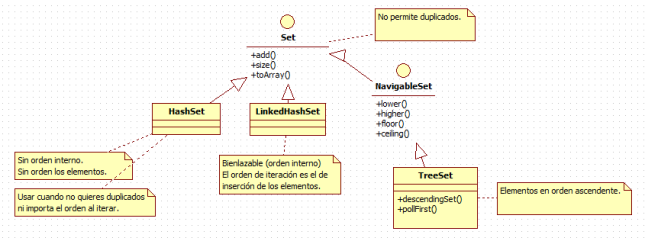
\includegraphics[scale=0.55]{imagenes/set.png}
\end{figure}
\end{frame}

\begin{frame}
\frametitle{Interfaz Set}
\begin{itemize}[<+->]
\item Cada elemento que se añada al objeto \emph{Set} debe ser único.
\item Si no es así \emph{Set} no añade el elemento duplicado.
\item Los objetos añadidos a un \emph{Set} debe implementar \emph{equals} para establecer la unicidad de los objetos.
\item No se garantiza que los elementos se guarden en un orden particular.
\end{itemize}
\pause
\begin{block}{Algunos metodos}
\begin{multicols}{2}
\begin{itemize}[<+->]
\item boolean add(Object)
\item boolean addAll(Collection)
\item void clear()
\item boolean contains(Object)
\item boolean containsAll(Collection)
\item boolean isEmpty()
\item boolean remove(Object)
\item boolean removeAll(Collection)
\item int size()
\item Object[] toArray()
\end{itemize}
\end{multicols}
\end{block}
\end{frame}

\begin{frame}
\frametitle{Clase HashSet}
\begin{itemize}[<+->]
\item Se puede utilizar para implementar la interfaz SET.
\item Implementa la interface SET basada en una tabla hash 
\item Una tabla hash será una tabla que se construye en base a claves que permiten localizar objetos.
\item Esta clase sea ideal para búsqueda, inserción y borrado de elementos.
\item No hay garantía de orden.
\item Se permite el uso de elementos nulos.
\item Esta clase no está sincronizada.
\item Si varios hilos intentan acceder al HashSet, este debe sincronizarse externamente:
\item Set s = Collections.synchronizedSet(new HashSet(\dots));
\end{itemize}
\end{frame}

\begin{frame}[fragile]
\frametitle{Ejemplo}
\begin{multicols}{2}
\begin{tiny}
\begin{verbatim}
public class Persona
{
  public int dni;
  public String nombre;
  public Persona (int d, String n)
  {
    this.dni = d;
    this.nombre = n;
  }
  @Override
  public int hashCode() {
    final int prime = 31;
    int result = 1;
    result = prime * result + dni;
    return result;
   }
        @Override

  public boolean equals (Object o)
  {
    return this.dni == ((Persona)o).dni;

  }
  public String toString ()
  {
    return "Persona: " + this.nombre;
  }
}



import java.util.Set;
import java.util.HashSet;
public class TestSetPersona
{
  public static void main (String[]arg)
  {
    Set < Persona > s = new HashSet < Persona > ();
    Persona p1 = new Persona (11111111, "juan");
    Persona p2 = new Persona (22222222, "luis");
    Persona p3 = new Persona (33333333, "lorenzo");
      s.add (p1);
      s.add (p2);
      s.add (p3);
      System.out.println (s);
      System.out.println (s.contains (p1));
    for (Persona p:s)
      {
        System.out.println (p);
        System.out.println (p.hashCode ());
      }

    Object[] p = s.toArray ();
  for (Object o:p)
      {
        System.out.println ((Persona) o);
        System.out.println (((Persona) o).hashCode ());
      }
  }
}
\end{verbatim}
\end{tiny}
\end{multicols}
\end{frame}



\begin{frame}
\frametitle{Metodo hashCode}
\begin{itemize}[<+->]
\item Un HashCode es un identificador de 32 bits que se almacena en un Hash en la instancia de la clase.
\item Es la dirección de memoria del objeto en hexadecimal.
\item Toda clase debe proveer de un método hashCode() que permite recuperar el Hash Code asignado, por defecto, por la clase Object. 
\item  El HashCode tiene una especial importancia para el rendimiento de las tablas Hash y otras Estructura de datos que agrupan objetos en base al cálculo de los HashCode.
\item Todas las clases heredan de java.lang.Object un sistema básico para el uso de hash, aunque es común sobreescribir este para obtener una función hash que maneje de forma más especifica los datos contenidos.
\item Normalmente se sobrescribe el método para que se comporte de forma acorde a la que lo hace .equal(), es decir, si el método .equals() dice que dos objetos son iguales, estos han de tener el mismo valor hash.


\end{itemize}
\end{frame}

\begin{frame}[fragile]
\frametitle{Ejemplo de hasCode sin sobrescribir}
\begin{tiny}
\begin{verbatim}
public class Demo{
  private int boleta;
  public Demo (int boleta)
  {
    this.boleta = boleta;
  }
  public int getBoleta ()
  {
    return this.boleta;
  }
  @Override public boolean equals (Object o)
  {
    if ((o instanceof Demo) && (((Demo) o).getBoleta () == this.boleta))
      {
        return true;
      }
    else
      {
        return false;
      }
  }
  public static void main (String[]args)
  {
    Demo demoA = new Demo (20);
    Demo demoB = new Demo (20);
    System.out.println (demoA.equals (demoB));
    System.out.println (demoA.hashCode ());
    System.out.println (demoB.hashCode ());
  }
}
                             DEVUELVE:
                                true
                                325040804
                                1173230247
\end{verbatim}
\end{tiny}
\end{frame}

\begin{frame}[fragile]
\frametitle{Ejemplo de hasCode sobrescrito}
\begin{tiny}
\begin{multicols}{2}
\begin{verbatim}
public class Demo1
{
  private int boleta;
  public Demo1 (int boleta)
  {
    this.boleta = boleta;
  }
  public int getBoleta ()
  {
    return this.boleta;
  }
  @Override public boolean equals (Object o)
  {
    if ((o instanceof Demo) && 
       (((Demo) o).getBoleta () == this.boleta))
      {
        return true;
      }
    else
      {
        return false;
      }
  }
  @Override public int hashCode ()
  {

    int hash = 7;

    hash = 97 * hash + this.boleta;

    return hash;

  }
  public static void main (String[]args)
  {
    Demo1 demoA = new Demo1 (20);
    Demo1 demoB = new Demo1 (20);

    System.out.println (demoA.equals (demoB));
    System.out.println (demoA.hashCode ());
    System.out.println (demoB.hashCode ());
  }
}

     DEVUELVE:
      true
      699
      699
\end{verbatim}
\end{multicols}
\end{tiny}
\end{frame}

\begin{frame}
\frametitle{TreeSet}
\begin{itemize}[<+->]
\item Esta implementación está basada en el uso de una estructura de árbol.
\item Permitiendo que los elementos estén ordenados bien por orden natural o bien por orden total definido por un Comparator.
\item Es muy rápido para búsquedas, inserciones y borrados de sus elementos.
\item La diferencia principal de esta clase con HashSet es que sus elementos están ordenados.
\item Otra diferencia es la estructura de datos que sirve para almacenar datos, en un caso una tabla y en otro un árbol.	
\end{itemize}
\pause
\begin{block}{Algunos metodos}
\begin{multicols}{2}
\begin{footnotesize}
\begin{itemize}[<+->]
\item public E first()
\item public E last()
\item public SortedSet$<E>$ tailSet(E fromElement)
\item public SortedSet$<E>$ headSet(E toElement)
\item public E lower(E e)
\item public E floor(E e)
\item public E ceiling(E e)
\item public E higher(E e)
\item public E pollFirst()
\item public E pollLast()
\end{itemize}
\end{footnotesize}
\end{multicols}
\end{block}
\end{frame}

\begin{frame}[fragile]
\frametitle{Ejemplo TreeSet}
\begin{tiny}
\begin{verbatim}
import java.util.Iterator;
import java.util.TreeSet;
public class TreeSetExample {
   public static void main(String[] args) {
        System.out.println("Tree Set Example!\n");
        TreeSet<Integer> tree = new TreeSet<Integer>();
        tree.add(12);tree.add(63);tree.add(34);tree.add(45);
        Iterator<Integer> iterator = tree.iterator();
        System.out.print("Tree set data: ");
        while (iterator.hasNext()) {
                System.out.print(iterator.next() + " ");}
        System.out.println();
        if (tree.isEmpty()) {
                System.out.print("Tree Set is empty.");
        } else {System.out.println("Tree Set size: " + tree.size());}
        System.out.println("First data: " + tree.first());
        System.out.println("Last data: " + tree.last());
        if (tree.remove(45)) { // remove element by value
                System.out.println("Data is removed from tree set");
        } else {System.out.println("Data doesn't exist!");}
        System.out.print("Now the tree set contain: ");
        iterator = tree.iterator();
        while (iterator.hasNext()) {System.out.print(iterator.next() + " ");}
        System.out.println();
        System.out.println("Now the size of tree set: " + tree.size());
        tree.clear();
        if (tree.isEmpty()) {
                System.out.print("Tree Set is empty.\n");
        } else {System.out.println("Tree Set size: \n" + tree.size());}
   }
}
\end{verbatim}
\end{tiny}
\end{frame}

%\subsection{La interfaz Map}
\begin{frame}[fragile]
\frametitle{La clase HasMap}
\begin{itemize}[<+->]
\item Esta clase y las derivadas vienen a reemplazar la antigua clase Dictionary.
\item HashMap$<K,V>$ es el tipo de mapeo más sencillo y probablemente el más usado.
\item Es la clase a utilizar si queremos asociar pares de claves y valores sin orden.
\item Utiliza un hash para almacenar la clave.
\item Una tabla hash se puede ver como un conjunto de entradas.
\item  Cada una de estas entradas tiene asociada una clave única, y por lo tanto, diferentes entradas de una misma tabla tendrán diferentes claves.
Esto implica, que una clave identifica univocamente a una entrada en una tabla hash.
\item No permite claves duplicadas, pero si utilizar null como clave.
\end{itemize}
\pause
\begin{verbatim}
     HashMap hashMap = new HashMap();
       hashMap.put("1","valor1");
       hashMap.put("2","valor2");
       hashMap.put("3","valor3");
\end{verbatim}
\end{frame}

\begin{frame}
\frametitle{La clase Hashtable}
\begin{itemize}[<+->]
\item Esta clase es muy similar a HashMap$<K,V>$
\item Con la excepción de que es sincronizada y que no acepta utilizar el valor null como clave.
\item Nos interesará utilizar HashMap$<K,V>$ siempre que no estemos utilizando varios hilos de ejecución.
\item En el caso de que necesitemos sincronización, otra opción es utilizar el método Collections.synchronizedMap sobre un HashMap.
\end{itemize}
\end{frame}

\begin{frame}
\frametitle{La clase LinkedHashMap}
\begin{itemize}[<+->]
\item LinkedHashMap$<K,V>$ es una clase introducida con el J2SE 1.4 que extiende HashMap$<K,V>$ 
\item Utiliza una lista doblemente enlazada para poder recorrer los elementos de la colección en el orden en el que se añadieron.
\item Esta clase es ligeramente más rápida que HashMap$<K,V>$ a la hora de acceder a los elementos, pero es algo más lenta al añadirlos.
\end{itemize}
\end{frame}

\begin{frame}
\frametitle{La clase TreeMap}
\begin{itemize}[<+->]
\item TreeMap$<K,V>$, en el que los pares clave-valor se almacenan en un árbol ordenado según los valores de las claves.
\item La clase es más lenta a la hora de añadir nuevos elementos, pero también a la hora de accederlos.
\end{itemize}
\end{frame}

\begin{frame}
\frametitle{Métodos mas comunes}
\begin{itemize}[<+->]
\item void clear(): Elimina todos los elementos de la colección.
\item boolean containsKey(Object key): Comprueba si la clave especificada se encuentra en la colección.
\item boolean containsValue(Object value): Comprueba si el valor especificado se encuentra en la colección.
\item V get(Object key): Devuelve el valor asociado a la clave especificada o null si no se encontró.
\item boolean isEmpty(): Comprueba si la colección está vacía.
\item Set keySet(): Devuelve un conjunto con las claves contenidas en la colección.
\item V put(K key, V value): Añade un nuevo par clave-valor a la colección.
\item V remove(Object key): Elimina el par clave-valor correspondiente a la clave pasada como parámetro.
\item int size(): Devuelve el número de pares clave-valor que contiene la colección.
\item Collection values(): Devuelve una colección con los valores que contiene la colección.
\end{itemize}
\end{frame}

\begin{frame}[fragile]
\frametitle{Ejemplo de HashMap}
\begin{tiny}
\begin{verbatim}
import java.util.Map;
import java.util.HashMap;
public class Alumnos
{
  private int age;
  private String name;

    Alumnos (String name, int age)
  {
    this.name = name;
    this.age = age;
  }
}
class TestAlumnos
{
  public static void main (String[]arg)
  {
    Alumnos person1 = new Alumnos ("Juan", 14);
    Alumnos person2 = new Alumnos ("Felix", 15);
      Map < Alumnos, String > m = new HashMap < Alumnos, String > ();
      m.put (person1, "valor1");
      m.put (person2, "valor2");
      System.out.println (m);
      System.out.println (m.keySet ());
      System.out.println (m.size ());
  }
}
\end{verbatim}
\end{tiny}
\end{frame}

\begin{frame}[fragile]
\frametitle{Ejemplo de Hashtable}
\begin{tiny}
\begin{verbatim}
import java.util.*;

public class Direccion
{
  public static void main (String[]args)
  {

    Hashtable direccion = new Hashtable ();

    Integer ocho = new Integer (8000);
      direccion.put ("calle", "Primavera");
      direccion.put ("numero", ocho);
      direccion.put ("colonia", " La Silla ");
      direccion.put ("ciudad", " Monterrey ");
      direccion.put ("estado", " Nuevo Leon ");
      direccion.put ("pais", "Mexico");

      String miciudad = (String) direccion.get ("ciudad");
      String miestado = (String) direccion.get ("estado");
      String micalle = (String) direccion.get ("calle");
      Integer minumero = (Integer) direccion.get ("numero");

      System.out.println ("Direccion : " + micalle + " " + minumero);
      System.out.println ("Lugar: " + miciudad + "," + miestado);

  }
}
\end{verbatim}
\end{tiny}
\end{frame}

\begin{frame}[fragile]
\frametitle{Ejemplo de LinkedHashMap}
\begin{tiny}
\begin{verbatim}
import java.util.*;

public class LinkedHashMapDemo {

   public static void main(String args[]) {
      // Create a hash map
      LinkedHashMap lhm = new LinkedHashMap();
      // Put elements to the map
      lhm.put("Zara", new Double(3434.34));
      lhm.put("Mahnaz", new Double(123.22));
      lhm.put("Ayan", new Double(1378.00));
      lhm.put("Daisy", new Double(99.22));
      lhm.put("Qadir", new Double(-19.08));
      
      // Get a set of the entries
      Set set = lhm.entrySet();
      // Get an iterator
      Iterator i = set.iterator();
      // Display elements
      while(i.hasNext()) {
         Map.Entry me = (Map.Entry)i.next();
         System.out.print(me.getKey() + ": ");
         System.out.println(me.getValue());
      }
      System.out.println();
      // Deposit 1000 into Zara's account
      double balance = ((Double)lhm.get("Zara")).doubleValue();
      lhm.put("Zara", new Double(balance + 1000));
      System.out.println("Zara's new balance: " +
      lhm.get("Zara"));
   }
}
\end{verbatim}
\end{tiny}
\end{frame}

\begin{frame}
\frametitle{Diferencias en los Hash}
\begin{description}
\item[HashMap:] carece totalmente de orden, no tiene nada que ver el orden con el que insertas los elementos al orden con el que los extraes…
\item[TreeMap:] al extraer los elementos lo hace siguiendo un “orden natural” de claves segun su método compareTo() (También se puede usar un Comparator). Adicionalmente implementa la interface de SortedMap que contiene métodos que dependen del orden.
\item[LinkedHashMap:] se iran extrayendo los elementos en el mismo orden con el que se fueron insertando en el map.
\end{description}
\end{frame}

\begin{frame}
\frametitle{Iterator}
\begin{itemize}[<+->]
\item Se Utiliza para recorrer colecciones.
\item Permite eliminar elementos de la colección.
\item Métodos que implementa la interfaz:
\begin{description}
\item[boolean hasNext()] devuelve true si quedan mas elementos en la colección.
\item[E next()] devuelve el elemento de tipo \emph{E} de la colección.
\item[void remove()] elimina el elemento de la colección sobre la que se está iterando.
\end{description}
\end{itemize}
\end{frame}

\begin{frame}[fragile]
\frametitle{Ejemlo de Iterator}
\begin{tiny}
\begin{verbatim}
import java.util.List;
import java.util.Arrays;
import java.util.ArrayList;
import java.util.Iterator;
public class IteratorHowTo
{
  public static void main (String args[])
  {
    List < String > androidVersions =
      Arrays.asList ("Petit Four", "Cupcake", "Donut",
                     "Eclair", "Froyo", "Gingerbread",
                     "Honeycomb", "Ice Cream Sandwich", "Jelly Bea");

    List < String > android = new ArrayList < String > (androidVersions);
    //Getting Iterator from List
    Iterator < String > iterator = android.iterator ();
    System.out.println ("Size of List before Iteratation " + android.size ());
    //Using Iterator to iterate over List, acces object one by one
    while (iterator.hasNext ())
      {
        String version = iterator.next ();
          System.out.println (version);
          iterator.remove ();   // you should be using Iterator's remove method
      }

    System.out.
      println ("Size of list after removing object during Iteration : " +
               android.size ());
  }
}
\end{verbatim}
\end{tiny}
\end{frame}


\begin{frame}
\frametitle{Resumen}
\begin{footnotesize}
\begin{itemize}[<+->]
\item Un \alert{array} asocia indices numericos a objetos. Guarda objetos de un tipo. Puede guardar datos primitivos. Pero no puede cambiar su tamaño una vez creado.
\item Una \alert{Collection} guarda elementos sencillos, mientras que un \alert{Map} guarda pares asociados.
\item Como un \alert{array} una \alert{List} tambien asocia indices numericos a los objetos. \alert{List} se redimensiona automaticamente. Una \alert{List} solo guarda referencias a objetos por lo que no puede guardar datos primitivos.  
\item Cuando se hace muchos accesos aleatorios se suele usar \alert{ArrayList} y una \alert{LinkedList} si se esta haciendo muchas inserciones y eliminaciones del medio de la lista.
\item El comportamiento de colas y pilas se proporciona con \alert{LinkedList}.
\item Un \alert{HashMap} se centra en el acceso rapido mientras que un \alert{TreeMap} mantiene sus claves ordenadas, no siendo tan rapido como un \alert{HashMap}
\item Un \alert{Set} solo acepta objetos diferentes. Los \alert{HashSet} proporciona busquedas extremadamente rapidas, mientras que los \alert{TreeSet} mantiene los elementos ordenados.
\item No hay necesidad de usar clases antiguas como \alert{Vector}, \alert{HashTable} y \alert{Stack}
\end{itemize}
\end{footnotesize}
\end{frame}

\begin{frame}
\frametitle{FIN}
\begin{figure}

\includegraphics[scale=0.4]{imagenes/end.png}
\end{figure}
\end{frame}

\end{document}